\documentclass[10pt,t]{beamer}

\begin{document}

\title{Development of a Computer Program for Electronic Structure
Calculation using Lagrange Basis Functions}
\author{Fadjar Fathurrahman and Hermawan K. Dipojono}
\institute{
Department of Engineering Physics, Institut Teknologi Bandung \\
Research Center for Nanoscience and Nanotechnology, Institut Teknologi Bandung
}
\date{29 November 2017}

\frame{\titlepage}

\begin{frame}[c]
\frametitle{Outline}

\begin{itemize}
\item Introduction
\item Kohn-Sham equations
\item Lagrange basis functions
\item Implementation
\item Numerical results
\end{itemize}

\end{frame}

\begin{frame}[c]
\frametitle{Introduction}

\begin{itemize}
\item Electronic structure calculations play important role for investigation of materials
properties.
\item Much of electronic structure calculations are based on Kohn-Sham density functional theory.
\item Several computer packages can already carry out electronic structure calculations
for systems containing of few atoms (characteristic length in angstrom) to ten thousands atoms
(10-$10^3$ nm)
\end{itemize}

{\centering
\includegraphics[scale=0.7]{images/web/SoftLogo.pdf}
\par}

\end{frame}


\begin{frame}[c]
\frametitle{Problems}

\begin{itemize}
\item These computer programs can "simplify" electronic structure calculations,
espescially for non-specialists.
However, they are not suitable for development of new methodologies.
It is quite difficult to extend the program if we want to do some customized calculations.
\item Much details are hidden beneath the programs. They usually contain thousands of lines codes
or more which can be very intimidating for beginner developers to work with.
\end{itemize}

\end{frame}



\begin{frame}[c]
\frametitle{This research}
  
\begin{itemize}
\item We will to write our own electronic structure calculations program.

\item \textbf{Downside}: It might takes several years to reach the same level
of maturity with state-of-the-art well-established electronic structure programs.

\item In this presentation, I will describe some of our preliminary works to implement
electronic calculation based on
{\color{blue}Kohn-Sham equations} and {\color{blue}Lagrange basis functions}
and results of the calculations for
{\color{blue}several simple systems}.
\end{itemize}


\end{frame}




\begin{frame}[c]
\frametitle{Kohn-Sham total energy functional}

Total energy of a system of interacting electrons according to Kohn-Sham
can be written as:
\begin{align*}
E_{\mathrm{tot}}\left[\{\psi_{i_{st}}(\mathbf{r})\},\rho(\mathbf{r})\right] & =
E_{\mathrm{kin}} + E_{\mathrm{ion}} + E_{\mathrm{Ha}} + E_{\mathrm{xc}} \\
%
\rho(\mathbf{r}) & = \sum_{i_{st} = 1}^{N_{st}} f_{i_{st}} \psi^{*}_{i_{st}}(\mathbf{r})
\psi_{i_{st}}(\mathbf{r}) \\
%
E_{\mathrm{kin}} & = -\frac{1}{2}\sum_{i_{st}}
\int f_{i_{st}}
\psi_{i_{st}}^{*}(\mathbf{r})\,\nabla^2\,\psi_{i_{st}}(\mathbf{r})
\,\mathrm{d}\mathbf{r} \\
%
E_{\mathrm{ion}} & = \int V_{\mathrm{ion}}(\mathbf{r})\, \rho(\mathbf{r})\,
\mathrm{d}\mathbf{r} \\
%
E_{\mathrm{Ha}} & = \frac{1}{2} \int 
\dfrac{\rho(\mathbf{r})\rho(\mathbf{r}')}
{\left|\mathbf{r} - \mathbf{r}'\right|}
\mathrm{d}\mathbf{r}\mathrm{d}\mathbf{r}' \\
%
E_{\mathrm{xc}} & = \int \epsilon_{\mathrm{xc}}\left[\rho(\mathbf{r})\right]
\rho(\mathbf{r})\,\mathrm{d}\mathbf{r}
\end{align*}

\end{frame}


\begin{frame}[c]
\frametitle{Kohn-Sham equations}

Ground state energy can be found by minimizing the Kohn-Sham energy functional or
by solving the Kohn-Sham equation:
\begin{equation}
\left[
-\frac{1}{2}\nabla^2  + V_{\mathrm{KS}}(\mathbf{r})
\right] \psi_{i_{st}}(\mathbf{r}) =
\epsilon_{i_{st}}\psi_{i_{st}}(\mathbf{r})
\end{equation}
with the following potential terms
\begin{align*}
V_{\mathrm{KS}}(\mathbf{r}) & = V_{\mathrm{ion}}(\mathbf{r}) + V_{\mathrm{Ha}}(\mathbf{r})
+ V_{\mathrm{xc}}(\mathbf{r}) \\
%
V_{\mathrm{Ha}}(\mathbf{r}) & = \int
\frac{\rho(\mathbf{r}')}
{\mathbf{r} - \mathbf{r}'}\,\mathrm{d}\mathbf{r}' \\
%
\nabla^{2} V_{\mathrm{Ha}}(\mathbf{r}) & = -4\pi \rho(\mathbf{r})
\end{align*}


\end{frame}


\begin{frame}[c]
\frametitle{Kohn-Sham equations}

\begin{itemize}
\item In the the implementation to solve Kohn-Sham equations, single-electron wave function must be
  represented as an expansion of basis functions or discretized using
  some discretization schemes such as finite-difference or finite-elements.
\item Several
  existing computer programs for DFT calculations, such as
  \textsc{Quantum Espresso} and \textsc{Gaussian09},
  expand single-electron wave function using plane wave and Gaussian functions, respectively.
\item Others, such as \textsc{Octopus} and \textsc{GPAW} use discretization based on finite-difference scheme.
\item In this work, we will use expansion based on Lagrange basis functions, which is relatively new
and currently there are no widely-available programs which implement this.
\end{itemize}

\end{frame}



\begin{frame}
\frametitle{Lagrange basis functions}

For a given interval $[0,L]$, with $L>0$, the grid points $x_{\alpha}$
appropriate for periodic Lagrange function are given by:

\begin{equation}
x_{\alpha}=\frac{L}{2}\frac{2\alpha-1}{N}
\end{equation}
with $\alpha=1,\ldots,N$. Number of points $N$ should be an odd number.

The periodic cardinal functions $\phi_{\alpha}(x)$, defined
at grid point $i$ are given by:
\begin{equation}
\phi_{\alpha}(x)=\frac{1}{\sqrt{NL}}\sum_{n=1}^{N}\cos\left(\frac{\pi}{L}(2n-N-1)(x-x_{\alpha})\right).
\end{equation}
The expansion of periodic function in terms of Lagrange functions:
\begin{equation}
f(x)=\sum_{\alpha=1}^{N}c_{\alpha}\phi_{\alpha}(x)
\end{equation}
with expansion coefficients $c_{\alpha}=\sqrt{L/N}f(x_{\alpha})$.

\end{frame}


\begin{frame}
\frametitle{Lagrange basis functions}

Plot of for Lagrange basis functions for $N = 5$, $L = 1.0$

{\centering
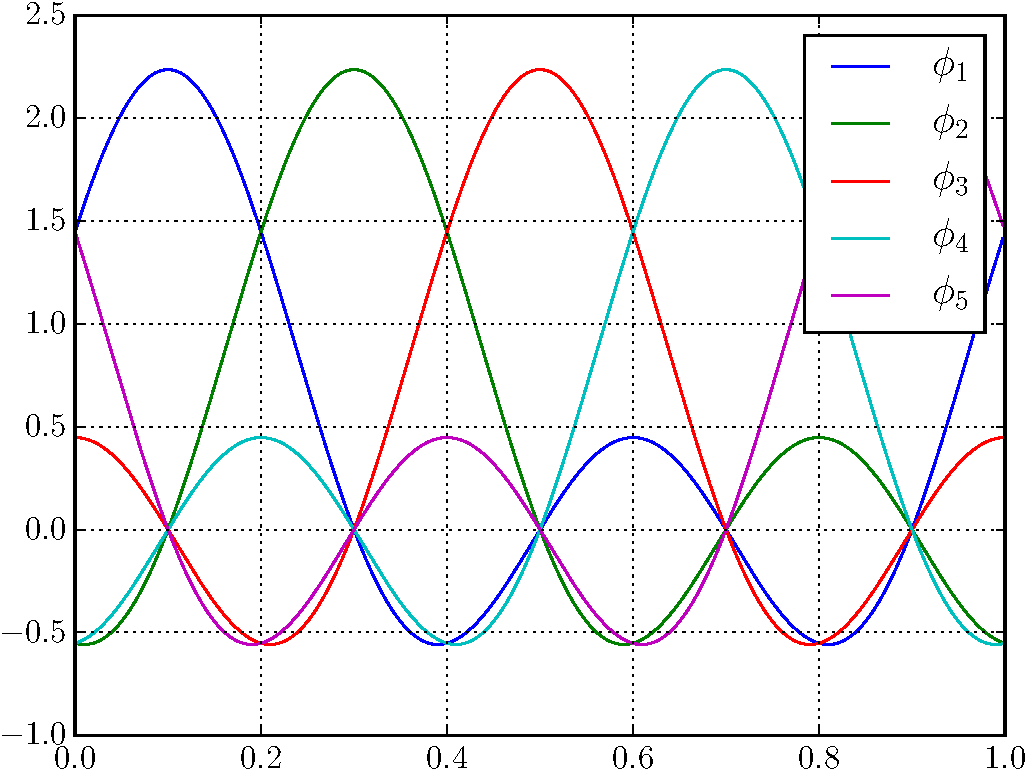
\includegraphics[scale=0.5]{images/plot_LF_p_N_5.pdf}
\par}

\end{frame}


\begin{frame}
\frametitle{Using Lagrange basis function for Schrodinger equation}

Given the 1D Schrodinger equation:
\begin{equation*}
\left[ -\frac{1}{2}\frac{\mathrm{d}^2}{\mathrm{d}x^2} + V(x)\right ] \psi(x)
= \epsilon \psi(x)
\end{equation*}
Lagrange basis function to expand the one-electron wavefunction:
\begin{equation*}
\psi(x) = \sum_{\alpha}^{N} c_{\alpha} \phi_{\alpha}(x)
\end{equation*}
Matrix equation:
\begin{equation*}
\left( \mathbf{T} + \mathbf{V} \right) \mathbf{C} = \epsilon \mathbf{C}
\end{equation*}

Analytic expression for matrix $\mathbf{T}$ can be obtained from reference
\footnote{See for example: \textit{J. Phys. Chem. A}
\textbf{110}, {5549-5560}, (2006)}.
Matrix $\mathbf{V}$ is diagonal.
Eigenvalue $\epsilon$ can be found using standard eigenvalue solver.

\end{frame}



\begin{frame}
\frametitle{Extension to 3D}

Expansion of function in 3D using Lagrange basis function:
\begin{equation*}
\psi(\mathbf{r} = (x,y,z)) =
\sum_{\alpha}\sum_{\beta}\sum_{\gamma} C_{\alpha\beta\gamma}
\phi_{\alpha}(x) \phi_{\beta}(y) \phi_{\gamma}(z)
\end{equation*}

Similar matrix equation can be obtained in 3D case.

Potential matrix is still diagonal and kinetic matrix now is expressed as:
\begin{equation*}
\mathbf{T}_{\alpha\beta\gamma}^{\alpha'\beta'\gamma'} =
\mathbf{T}_{\alpha\alpha'}\delta_{\beta\beta'}\delta_{\gamma\gamma'} +
\mathbf{T}_{\beta\beta'}\delta_{\alpha\alpha'}\delta_{\gamma\gamma'} +
\mathbf{T}_{\gamma\gamma'}\delta_{\alpha\alpha'}\delta_{\beta\beta'}
\end{equation*}
where $\mathbf{T}_{ii'}$, $i=\alpha,\beta,\gamma$ are kinetic matrix for 1D case.

Similar matrix representation can be found in for finite-difference methods
\footnote{See for example: \textit{Phys. Rev. Lett.} \textbf{72}, 1240 (1994).}.

Once we know how to calculate $\mathbf{T}$ and $\mathbf{V}$, we can find
solution to Kohn-Sham equations using standard self consistent cycle (SCF) procedure.

\end{frame}
  

\begin{frame}[c]
\frametitle{Numerical results}

We carry out total energy calculations for systems with the following
simple potentials:
\begin{itemize}
\item Gaussian potentials: convergence of total energy with respect to
grid spacing
\item atomic pseudotentials: hydrogen and lithium pseudopotentials
\end{itemize}

All calculations are done in $16\times16\times16$ bohr periodic box.
Center of the potential is set to the center of the box.

We will also validate the results of our program against result from
well-established program \textsc{Octopus} which uses finite difference method.

\end{frame}



\begin{frame}
\frametitle{Gaussian potentials}

\begin{equation*}
V^{\mathrm{Gau}}_{\mathrm{ion}}(r) = -A\exp(-\alpha r^2)
\end{equation*}

{
\centering
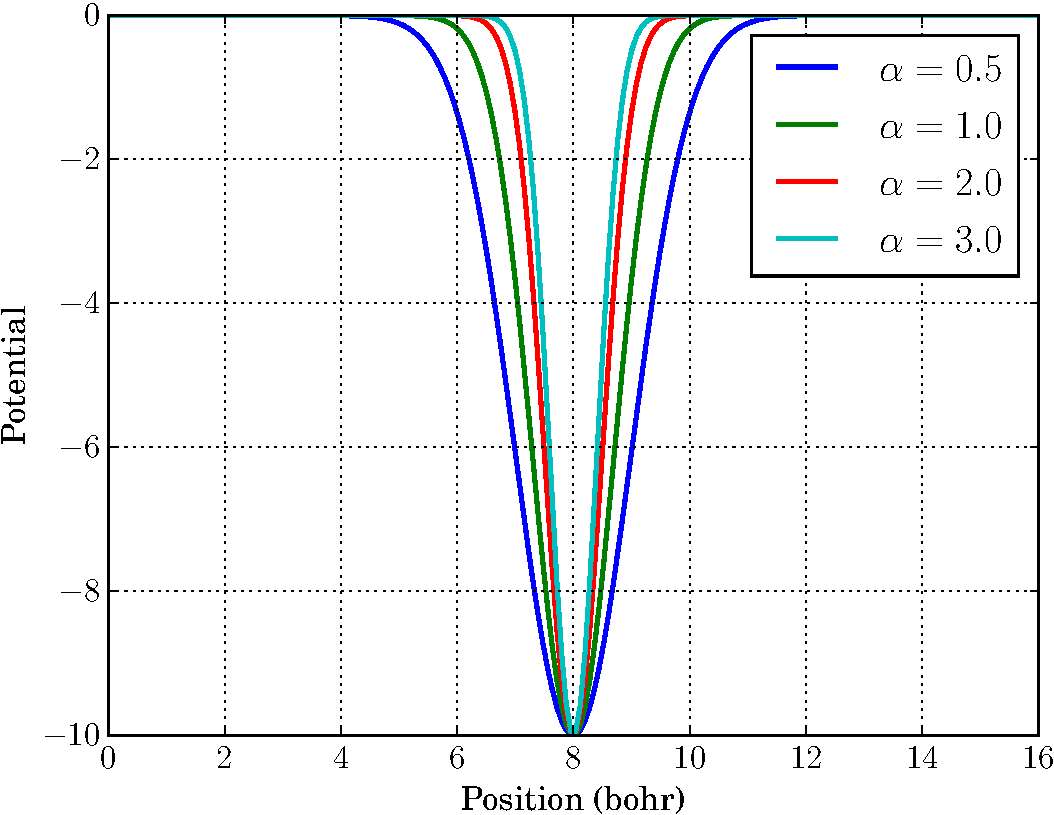
\includegraphics[scale=0.5]{images/V_gauss.pdf}
\par
}

\end{frame}


\begin{frame}
\frametitle{Total energy}  

{\centering
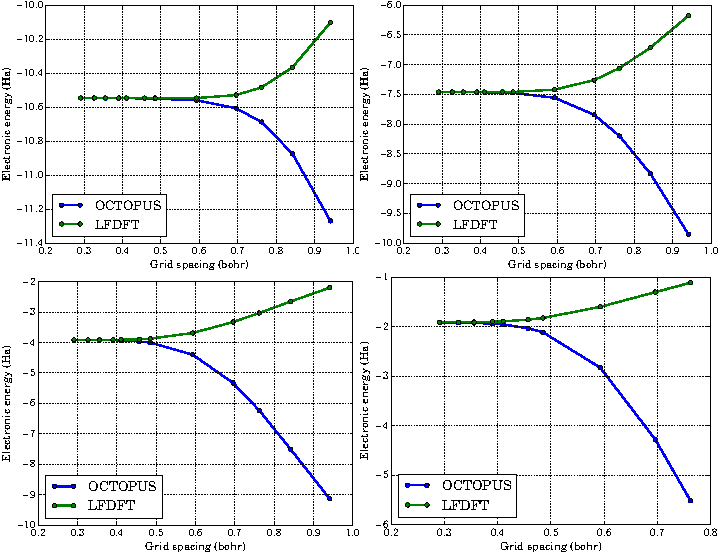
\includegraphics[width=0.8\textwidth]{images/COMBINE_v2.pdf}
\par
Both our program (LFDFT) and \textsc{Octopus} converge to the same total energy value
\par}

\end{frame}


\begin{frame}
\frametitle{Total energy convergence}

{\centering
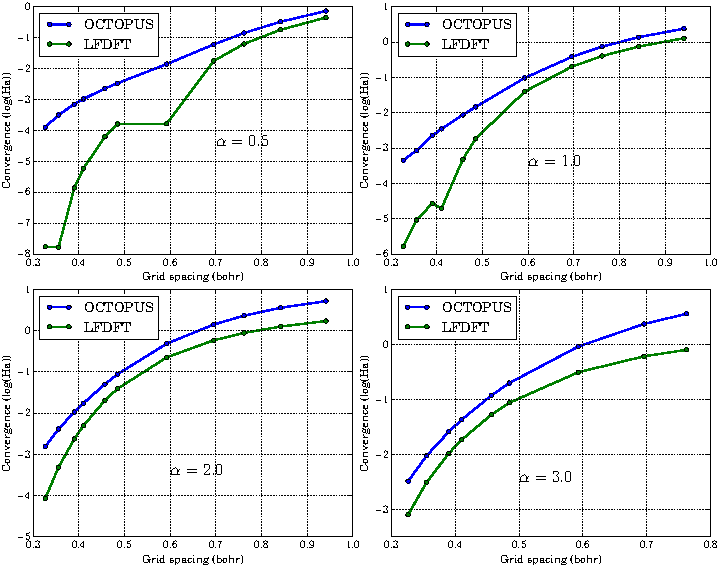
\includegraphics[width=0.8\textwidth]{images/COMBINE_v1.pdf}
\par
LFDFT converges faster than \textsc{Octopus} (finite difference)
\par
For smoother potential (smaller $\alpha$) both methods converge faster
(typicall for real-space methods)
\par}

\end{frame}



\begin{frame}
\frametitle{Hydrogen atom}

\begin{multline}
  V^{\mathrm{H}}_{\mathrm{loc}}(\mathbf{r}) = 
  -\dfrac{Z_{\mathrm{ion}}}{r}
  \mathrm{erf}\left(
  \dfrac{r}{\sqrt{2}r_{\mathrm{loc}}}
  \right) + \\
  \exp
  \left[ -\frac{1}{2}
  \left( \frac{r}{r_{\mathrm{loc}}}\right)^2
  \right]
  \times
  \left[
  C_{1} +
  C_{2}\left( \frac{r}{r_{\mathrm{loc}}}\right)^2 +
\right]
\end{multline}
with the following parameters:
$Z_{\mathrm{ion}} = 1$, $r_{\mathrm{loc}} = 0.2$,
$C_{1} = -4.1802372$, and $C_{2} = 0.725075$.
\footnote{
  \textit{Phys. Rev. B}  \textbf{58}, 3641 (1998). 
}

\end{frame}

\begin{frame}[plain,c]
  
{\centering
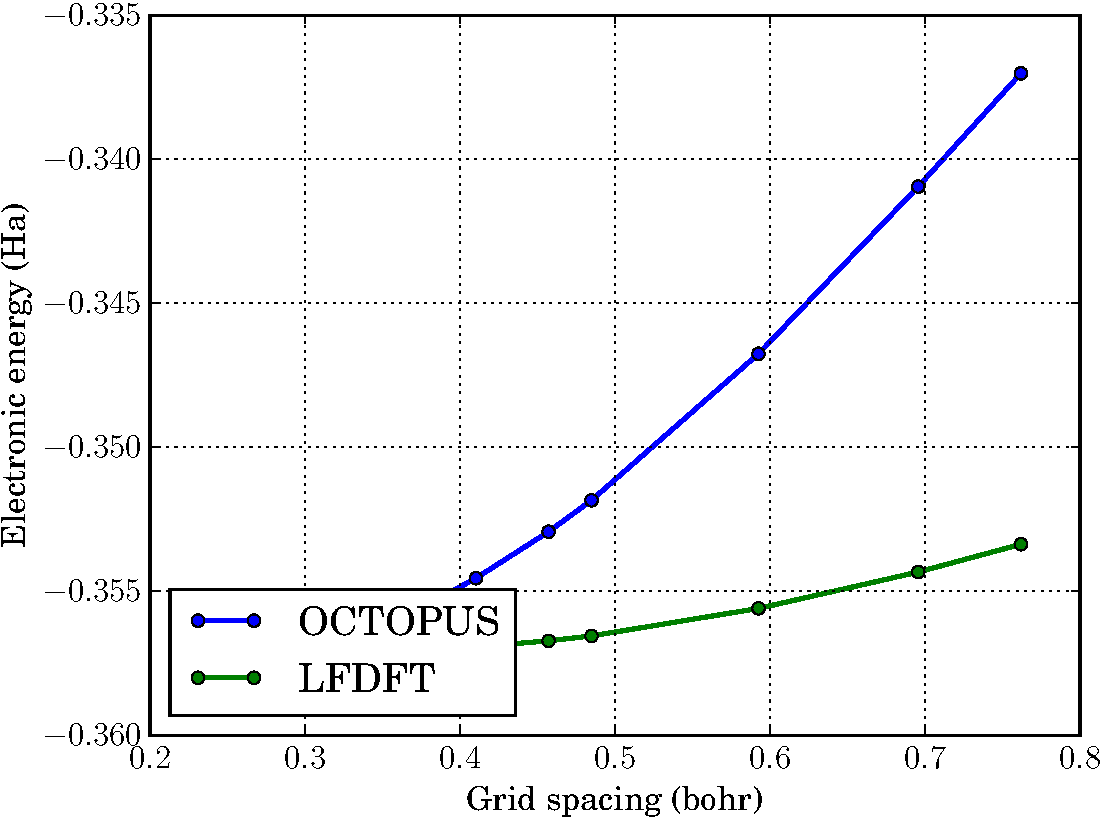
\includegraphics[width=0.45\textwidth]{images/atom_H.pdf}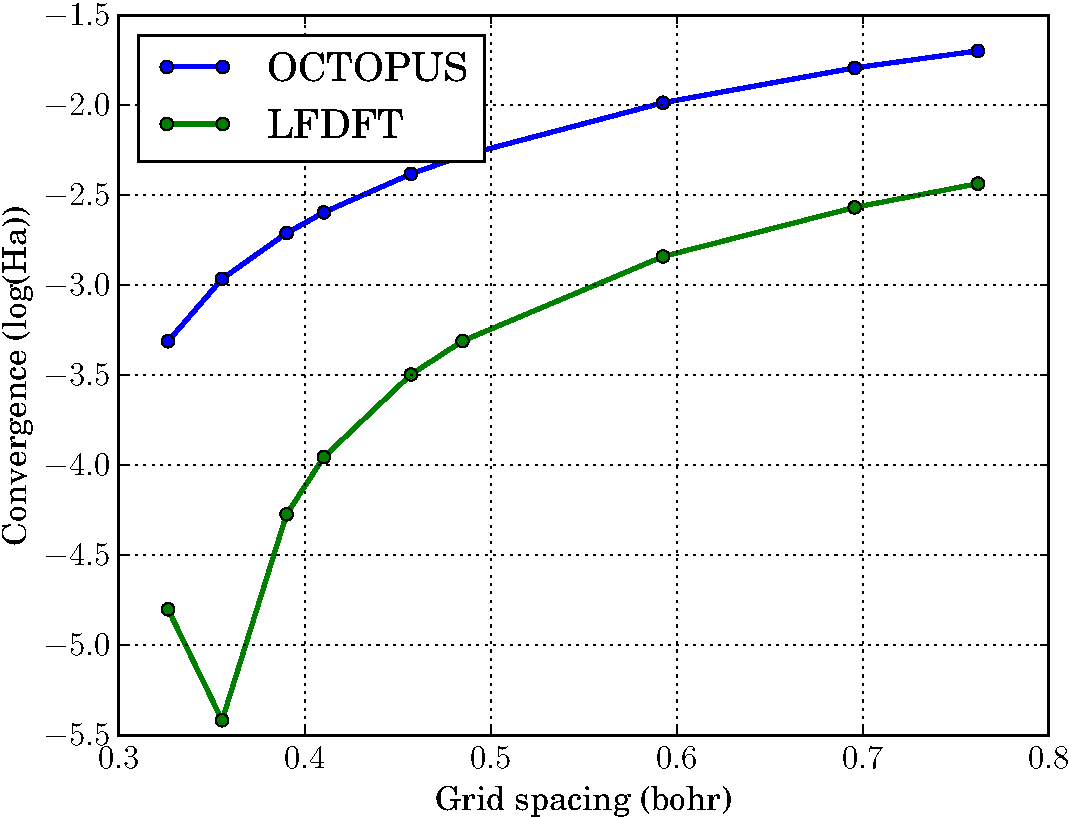
\includegraphics[width=0.45\textwidth]{images/CONV_atom_H.pdf}
\par
LFDFT converges faster than \textsc{Octopus} (finite difference)
\par}
  
\end{frame}


\begin{frame}
\frametitle{Lithium atom}

\begin{multline*}
V^{\mathrm{Li}}_{\mathrm{loc}}(\mathbf{r}) = 
-\dfrac{Z_{\mathrm{ion}}}{r}
\mathrm{erf}\left(
\dfrac{r}{\sqrt{2}r_{\mathrm{loc}}}
\right) + \\
\exp
\left[ -\frac{1}{2}
\left( \frac{r}{r_{\mathrm{loc}}}\right)^2
\right]
\times
\left[
C_{1} +
C_{2}\left( \frac{r}{r_{\mathrm{loc}}}\right)^2 +
C_{3}\left( \frac{r}{r_{\mathrm{loc}}}\right)^4 +
C_{4}\left( \frac{r}{r_{\mathrm{loc}}}\right)^6
\right]
\end{multline*}
with the following parameters:
$Z_{\mathrm{ion}} = 3$, $r_{\mathrm{loc}} = 0.4$,
$C_{1} = -14.034868$, $C_{2} = 9.553476$, $C_{3} = -1.7664885$
and $C_{4} = 0.084370$.
\footnote{
  \textit{Phys. Rev. B}  \textbf{58}, 3641 (1998). 
}


\end{frame}

\begin{frame}[c]
\frametitle{LiH HOMO and LUMO}

{\centering
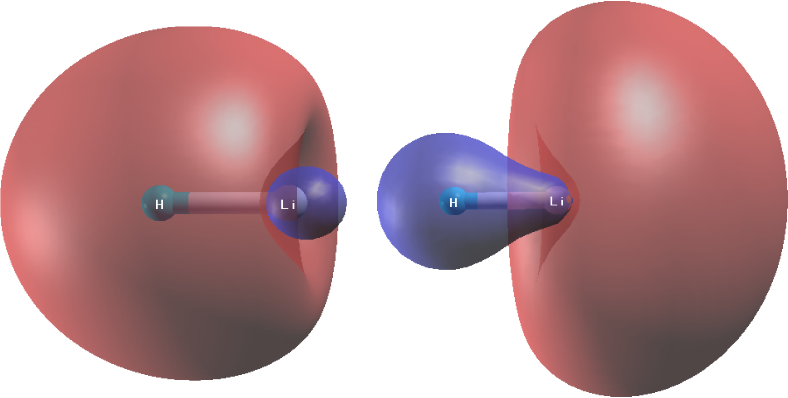
\includegraphics[scale=0.45]{images/LiH_HOMO_LUMO.png}
\par
HOMO (left image) and LUMO (right image) of LiH
\par}



\end{frame}

\begin{frame}[c]
\frametitle{Remarks and future works}

Remarks
\begin{itemize}
\item Use of Lagrange basis functions to Kohn-Sham equation gives
matrix-representation which is very similar to the one obtained by
using finite-difference methods
\item Compared to finite difference method, use of Lagrange basis functions
gives better total energy convergence with respect to grid size (number of basis
functions).
\end{itemize}

Future works will focus on:
\begin{itemize}
\item Larger systems
\item Paralellization
\end{itemize}

\end{frame}


\begin{frame}[c]
\frametitle{Thank you for your attention!}
    
Public repository: \url{https://github.com/f-fathurrahman/ffr-LFDFT}.
    
{\centering
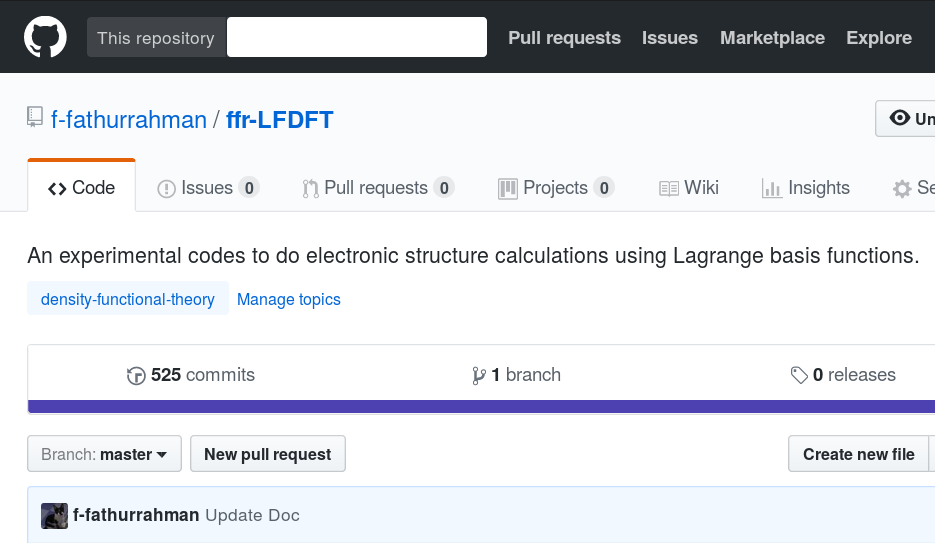
\includegraphics[scale=0.25]{images/ffr-LFDFT-github-cropped.png}
\par}

\end{frame}


\end{document}

